\chapter{Introducción}
\label{cap:introduccion}

\section{Contextualización}

Debido al avance de la tecnologı́a, cada vez disponemos de más dispositivos con la capacidad de capturar imágenes. Esto ha provocado un importante incremento en las bases de datos de imágenes, lo que a su vez ha propiciado la aparición de metodologı́as para solventar el problema de la manipulación, gestión y recuperación de dicha información. En este caso cuando hablamos de metodologı́as nos referimos a los sistemas de recuperación de información, basados fundamentalmente en descriptores de bajo nivel (color, textura, etc.) obtenidos directamente a partir de la imagen. Estos sistemas se denominan CBIR.\\

La recuperación de información es la actividad de obtener recursos de información relevantes para una necesidad de información a partir de una colección de recursos de información. Las búsquedas pueden ser basadas en texto, o en otro tipo de indexación basada en contenido. Para realizar esta actividad se utilizan los sistemas de recuperación de información, que se encargan de gestionar todo lo necesario.\\

Un proceso de recuperación de información comienza cuando un usuario realiza una consulta al sistema. Estas consultas son declaraciones de necesidad de información, por ejemplo, buscar una frase en un motor de búsqueda. Las consultas no identifican a un único objeto de la base de datos o colección, si no que afecta a varios con distintos grados de relevancia.\\

Un objeto, en este ámbito, es una entidad que representa la información en una colección o base de datos. Sin embargo, al contrario de lo que pasaría en una consulta a un sistema clásico SQL, los resultados son clasificados. Esta clasificación es la principal diferencia respecto a las búsquedas en bases de datos tradicionales.\\

Hay que tener en cuenta que dependiendo de la aplicación, los objetos pueden ser textos, imágenes, audio o vídeos, por ejemplo. La mayoría de los sistemas de recuperación de información manejan una puntuación numérico sobre como coincide cada objeto de la base de datos con el objeto consulta, y ordena los objetos acorde a este valor numérico. Los que se encuentran en las primeras posiciones del ranking se muestran al usuario.\\

Para realizar las consultas, los sistemas de recuperación utilizan los denonimados descriptores. Estos describen las características de los objetos que se encuentran en la colección de objetos accesibles por el sistema. Dado que en este trabajo nos vamos a centrar en un sistema de recuperación de información, vamos a hablar sobre sus mútliples descriptores, denominados descriptores visuales.\\

Estos descriptores representan características visuales de los objetos, siendo estos vídeos o imágenes. Describen características elementales como la forma, el color, o la textura, entre otros muchos.\\

Los descriptores visuales se encuentran divididos en dos grandes grupos:

\begin{itemize}

\item \textbf{Descriptores de información general}. Proporcionan descripciones sobre el color, formas, regiones y texturas.

\item \textbf{Desciptores de información de dominio específico}. Proporcionan información sobre sucesos que van apareciendo en escena. El reconocimiento de caras sería un ejemplo delimitado de este tipo.

\end{itemize}

\subsection{Descriptores de información general}

Como se ha mencionado, estos descriptores se encargan de representar distintas propiedades visuales elementales, como el color y la textura.

\subsubsection{Color}

Puede ser considerada como el atributo elemental del contenido visual. A continuación se especifican cinco formas para describir el color. Las tres primeras simbolizan la distribución del color. Las otras dos describen la distribución espacial del color y la relación del color en un conjunto o secuencia de imágenes.

\begin{itemize}
\item Dominant Color Descriptor (DCD)
\item Scalable Color Descriptor (SCD)
\item Color Structure Descriptor (CSD)
\item Color Layout Descriptor (CLD)
\item Group of frame (GoF) o Group-of-pictures (GoP)
\end{itemize}

\subsubsection{Textura}

Esta propiedad se encuentra desarrollada para caracterizar las regiones, o texturas de una imagen. Esto se lleva a cabo teniendo en cuenta la homogeneidad de las regiones y los histogramas de los bordes de esas regiones. Como representantes de este conjunto tenemos:

\begin{itemize}
\item Homogeneous Texture Descriptor (HTD)
\item Texture Browsing Descriptor (TBD)
\item Edge Histogram Descriptor (EHD)
\end{itemize}

\subsubsection{Forma}

En esta ocasión, estamos hablando de información semántica de gran relevancia, ya que los objetos son reconocidos visualmente por los seres humanos. La única manera de obtener dicha información es mediante la segmentación de la imagen. Desafortunadamente, aún no se encuentra completamente disponible, pero si disponemos de una serie de algoritmos que nos ofrecen buenas aproximaciones. Estos descriptores detallan formas, regiones y contornos, si hablamos de imágenes 2D, y volúmenes en el caso de 3D. Estos descriptores son:

\begin{itemize}
\item Region-based Shape Descriptor (RSD)
\item Contour-based Shape Descriptor (CSD)
\item 3-D Shape Descriptor (3-D SD)
\end{itemize}

 
Como se ha mencionado anteriormente, nos vamos a centrar en los sistemas de recuperación de imágenes, por lo que vamos a ver una serie de ejemplos sobre ellos.

\subsection{CBMIR}

Este CBIR es usado en ámbitos médicos, de ahí su nombre Content-based medical image retrieval, ha sido desarrollado por la universidad nacional de Malasia. Se centra en ayudar a diagnosticar irregularidades vertebrales, lo cual es muy importante si se realiza a tiempo para disminuir el riesgo de sufrir fracturas vertebrales. Las fracturas aparecen en radiografías, pero su detección es poco frecuente por parte de médicos y radiólogos. Por esta razón, el objetivo de este CBIR es ayudar al personal sanitario a detectar estas irregularidades como se ha comentado anteriormente.\\

Una vez definido este CBIR, veamos como visualiza la información de una consulta.\\

\begin{figure}[H] %con el [H] le obligamos a situar aquí la figura
\centering
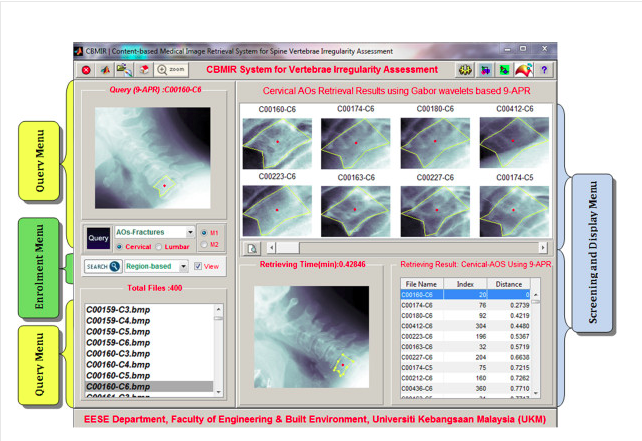
\includegraphics[scale=0.5]{imagenes/CBMIR.png}  %el parámetro scale permite agrandar o achicar la imagen. En el nombre de archivo puede especificar directorios
\label{CBMIR}
\caption{Sistema de recuperación de imágenes CBMIR}
\end{figure}

La visualización se realiza en la parte derecha de la pantalla. En la parte superior se aprecian todas las imágenes resultantes de la consulta, mientras que en la parte inferior podemos obtener mas información sobre cada una de esas imágenes.\\

Mientras que para la consulta se utiliza la parte izquierda. En ella se puede seleccionar el descriptor y la imagen a usar.\\

\subsection{Visual Clustering of Image Search Results}

La visulaización de ese sistema implementado por Trystan G. Upstill, Rajehndra Nagappan y Nick Craswellb se basa a su vez en un modelo primavera desarrollado por Olsen y Korfhage. Esta técnica fue adaptada de RadViz. En este sistema, RadViz, los puntos de referencia se distribuyen en torno de un círculo, mientras que los elementos de datos están distribuidos en el círculo según su atracción a los puntos de referencia.\\

En esta imágen se puede apreciar lo explicado:\\

\begin{figure}[H] %con el [H] le obligamos a situar aquí la figura
\centering
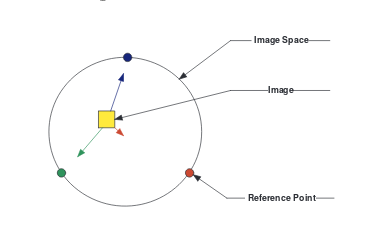
\includegraphics[scale=0.7]{imagenes/VCISR.png}  %el parámetro scale permite agrandar o achicar la imagen. En el nombre de archivo puede especificar directorios
\label{VCISR}
\caption{Puntos de atracción VCISR}
\end{figure}

Ahora veamos la representanción visual de una salida producida por una consulta.\\

\begin{figure}[H] %con el [H] le obligamos a situar aquí la figura
\centering
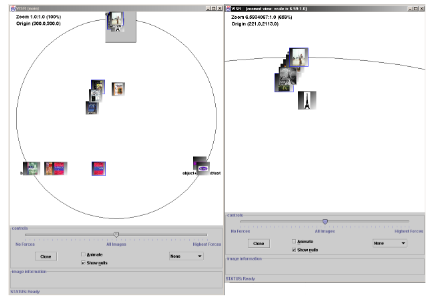
\includegraphics[scale=0.7]{imagenes/VCISR2.png}  %el parámetro scale permite agrandar o achicar la imagen. En el nombre de archivo puede especificar directorios
\label{VCISR}
\caption{Salida VCISR}
\end{figure}

Podemos apreciar como se distribuyen las imágenes a lo largo del círculo siguiendo el patrón comentado anteriormente.\\

Por otro lado podemos ver lo que ocurre al hacer zoom sobre una región. Al hacerlo apreciamos nuevas imágenes que permanecían ocultas.\\


\section{Fundamentos}

Este trabajo se basa en un sistema de recuperación de imágenes existente llamado \textit{Java Multimedia Retrival}, \textit{JMR}. Se trata de un \textit{CBIR} de código libre cuyo desarrollador principal e impulsor es el profesor Jesús Chamorro Martínez del departamento de Ciencias de la Computación e Inteligencia Artificial de la Universidad de Granada.\\

Se va hablar durante esta memoria sobre el espacio de color, por lo que es necesario darle una definición para saber a que nos referimos concretamente.\\

Por espacio de color nos referimos a un sistema de interpretación de color, una manera específica estructurar los colores de una imagen o vídeo. También es necesario hablar sobre los modelos de color, que se tratan de modelos matemáticos abstractos que describen la forma en la que cual los colores pueden ser representados como tuplas de números, normalmente como tres o cuatro valores o componentes de color, un ejemplo de esto sería RGB, en el que un color se descompone en tres valores, el valor de rojo, verde y azul.\\


\begin{figure}[H] %con el [H] le obligamos a situar aquí la figura
\centering
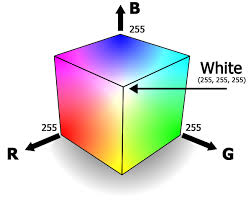
\includegraphics[scale=0.7]{imagenes/rgb.jpeg}  %el parámetro scale permite agrandar o achicar la imagen. En el nombre de archivo puede especificar directorios
\label{rgb.jpeg}
\caption{Modelo de color RGB}
\end{figure}

Otro ejemplo de espacio de color sería el \textit{HMMD}. Este espacio de color (Hue-Max-Min-Diff), es cercano a un espacio de color perceptualmente uniforme. Los nombres componentes, correspondientes a los distintos nombres, se pueden calcular a partir de RGB siguiente las siguientes transformaciones:

\begin{itemize}
\item \textbf{Max}: máximo(R,G,B)
\item \textbf{Min}: mínimo(R,G,B)
\item \textbf{Diff}: Max-min
\end{itemize}

Por otro lado, incluso se puede definir otro componente, llamado \texbf{Sum} = (Max+Min)/2.\\

En total habría una cantidad de 5 componentes en este espacio de color. Sin embargo, un cojunto de 3 elementos, {H,Max,Min} o {H,Diff,Sum}, es suficiente para para formar este espacio de color y especificar un punto de color.\\

\textit{Hue}, tiene la misma propiedad que su equivalente en el espacio de color HSV. \text{Hue} se mueve en el rango [0º, 360º]. \textit{Max} se mueve en el rango [0,1] y especifica cuanto color negro se encuentra presente, dando la sensación de sombra u oscuridad. \textit{Min}, rango [0,1], especifica cuanto color blanco se encuentra presente, dando la sensación de blanqueado. \textit{Diff}, rango [0,1], especifica como de cercano es un color a los colores puros, dando la sensación de tono o colorido. Finalmente, \textit{Sum}, especifica el brillo del color.
 
\begin{figure}[H] %con el [H] le obligamos a situar aquí la figura
\centering
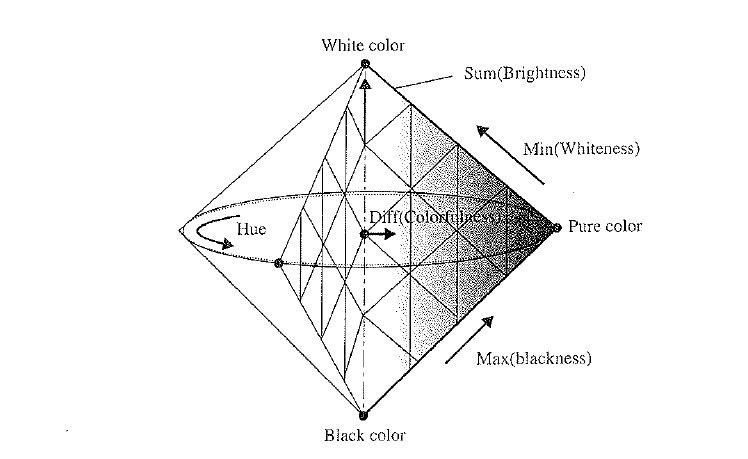
\includegraphics[scale=0.7]{imagenes/hmmd1.jpg}  %el parámetro scale permite agrandar o achicar la imagen. En el nombre de archivo puede especificar directorios
\label{hmmd1.jpg}
\caption{Modelo de color HMMD}
\end{figure}

\begin{figure}[H] %con el [H] le obligamos a situar aquí la figura
\centering
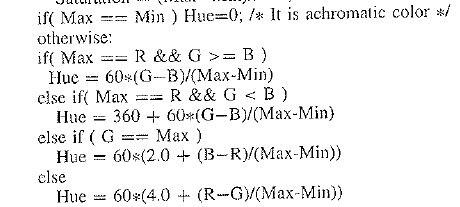
\includegraphics[scale=0.7]{imagenes/hmmd2.jpg}  %el parámetro scale permite agrandar o achicar la imagen. En el nombre de archivo puede especificar directorios
\label{hmmd2.jpg}
\caption{Cáculo Hue HMMD}
\end{figure}


Para este proyecto van a ser implementados una serie de descriptores. Estos descriptores se corresponden al tipo información general, previamente comentado, concretamente sobre el color. Estos son:

\begin{itemize}

\item Single Color Descriptor

\item MPEG7ColorStructure

\end{itemize}

\subsection{Single Color Descriptor}

Este descriptor de color se basa en el color medio de la imagen. Para calcularlo recorre una imagen en el espacio de color RGB pixel a pixel, obteniendo sus valores R, G y B. Cuando termina de recorrer todos los píxeles, calcula el color medio.

\subsection{MPEG7ColorStructure}







